\section{Introduction}
\begin{figure}[t]
\centering
    \begin{subfigure}[t]{\columnwidth}
    \centering
      \caption{Ainu (left) -- Japanese (right)}
      \vspace{-0.5em}
      \fbox{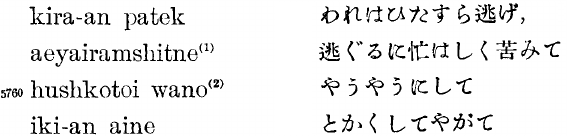
\includegraphics[width=0.9\columnwidth]{images/ainu_ex.png}}
      \vspace{0.6em}
    \end{subfigure}
    \begin{subfigure}[t]{\columnwidth}
      \centering
      \caption{Griko (top) -- Italian (bottom)}
      \vspace{-0.5em}
      \frame{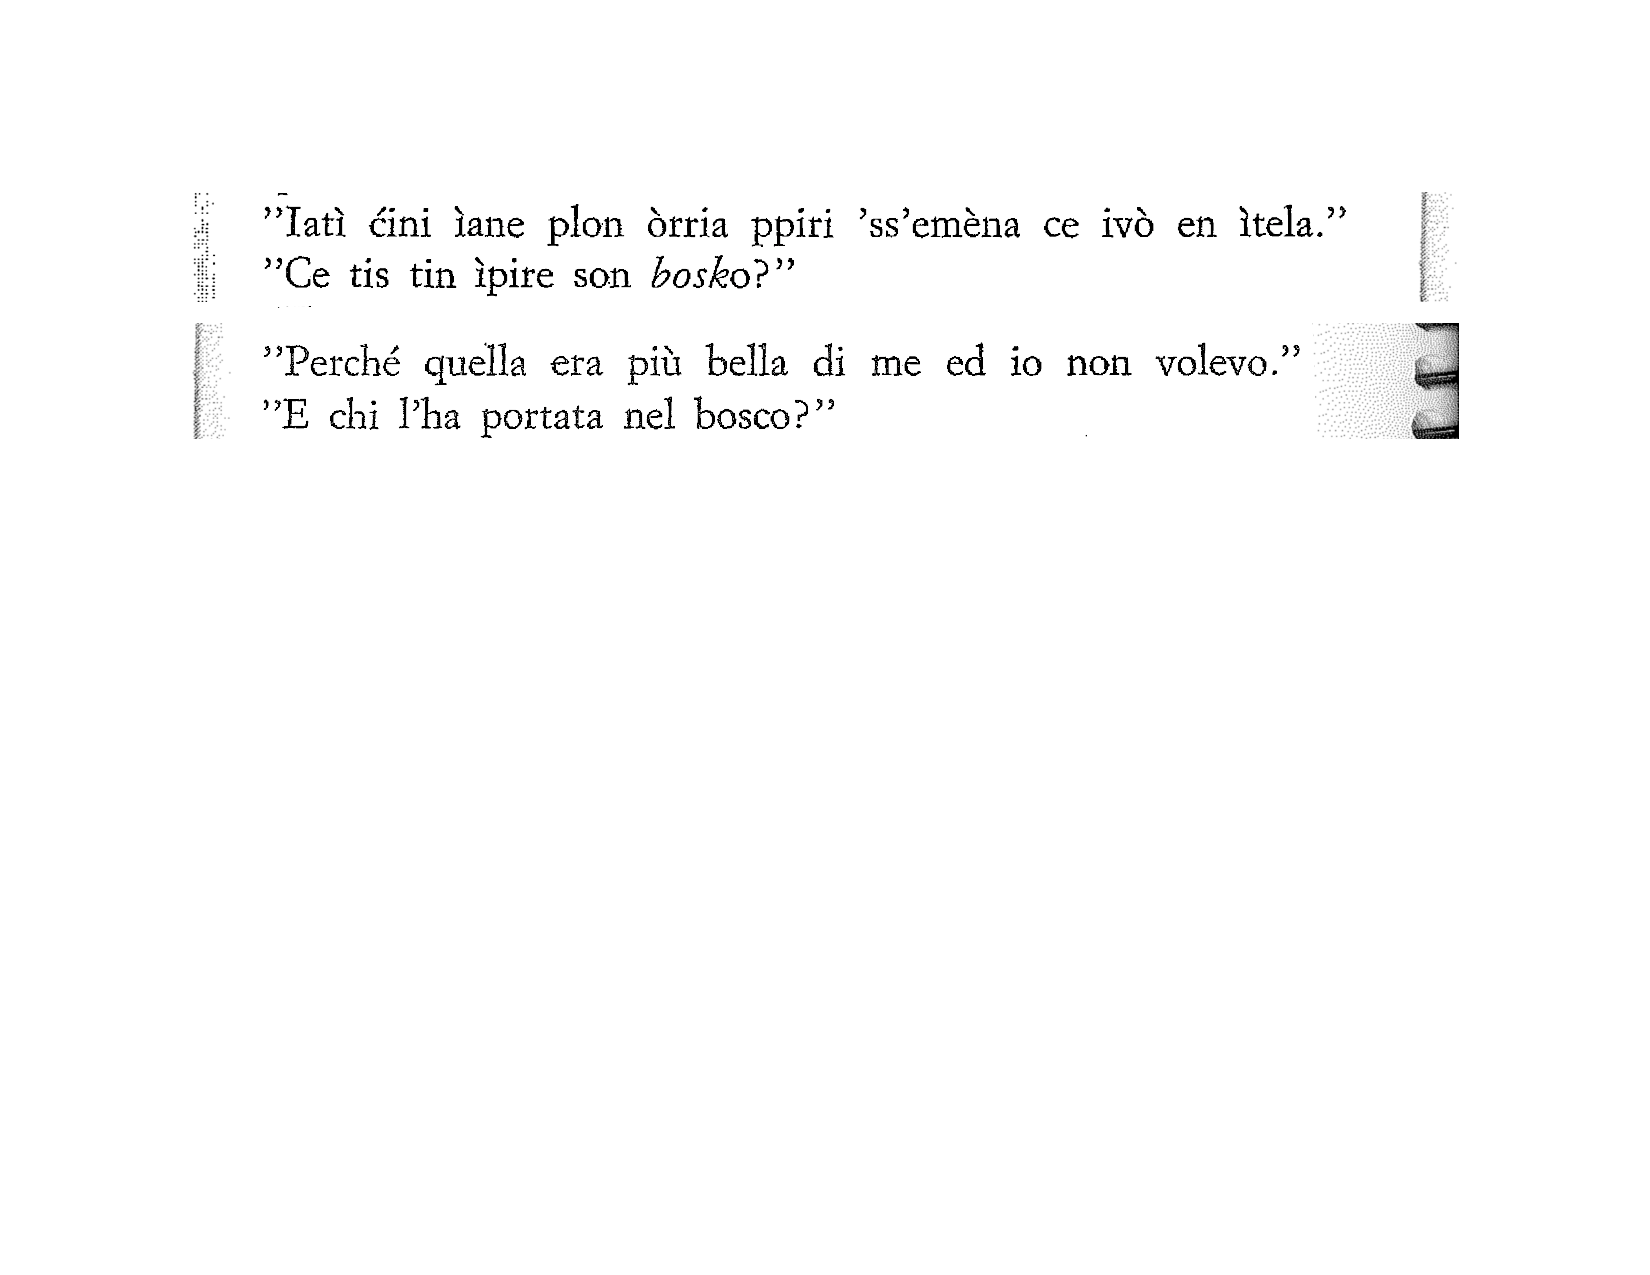
\includegraphics[width=0.93\columnwidth]{images/griko_example.pdf}}
      \vspace{0.7em}
    \end{subfigure}
    \begin{subfigure}[t]{\columnwidth}
      \centering
      \caption{Yakkha (top) -- Nepali (middle) -- English (bottom)}
      \vspace{-0.5em}
      \fbox{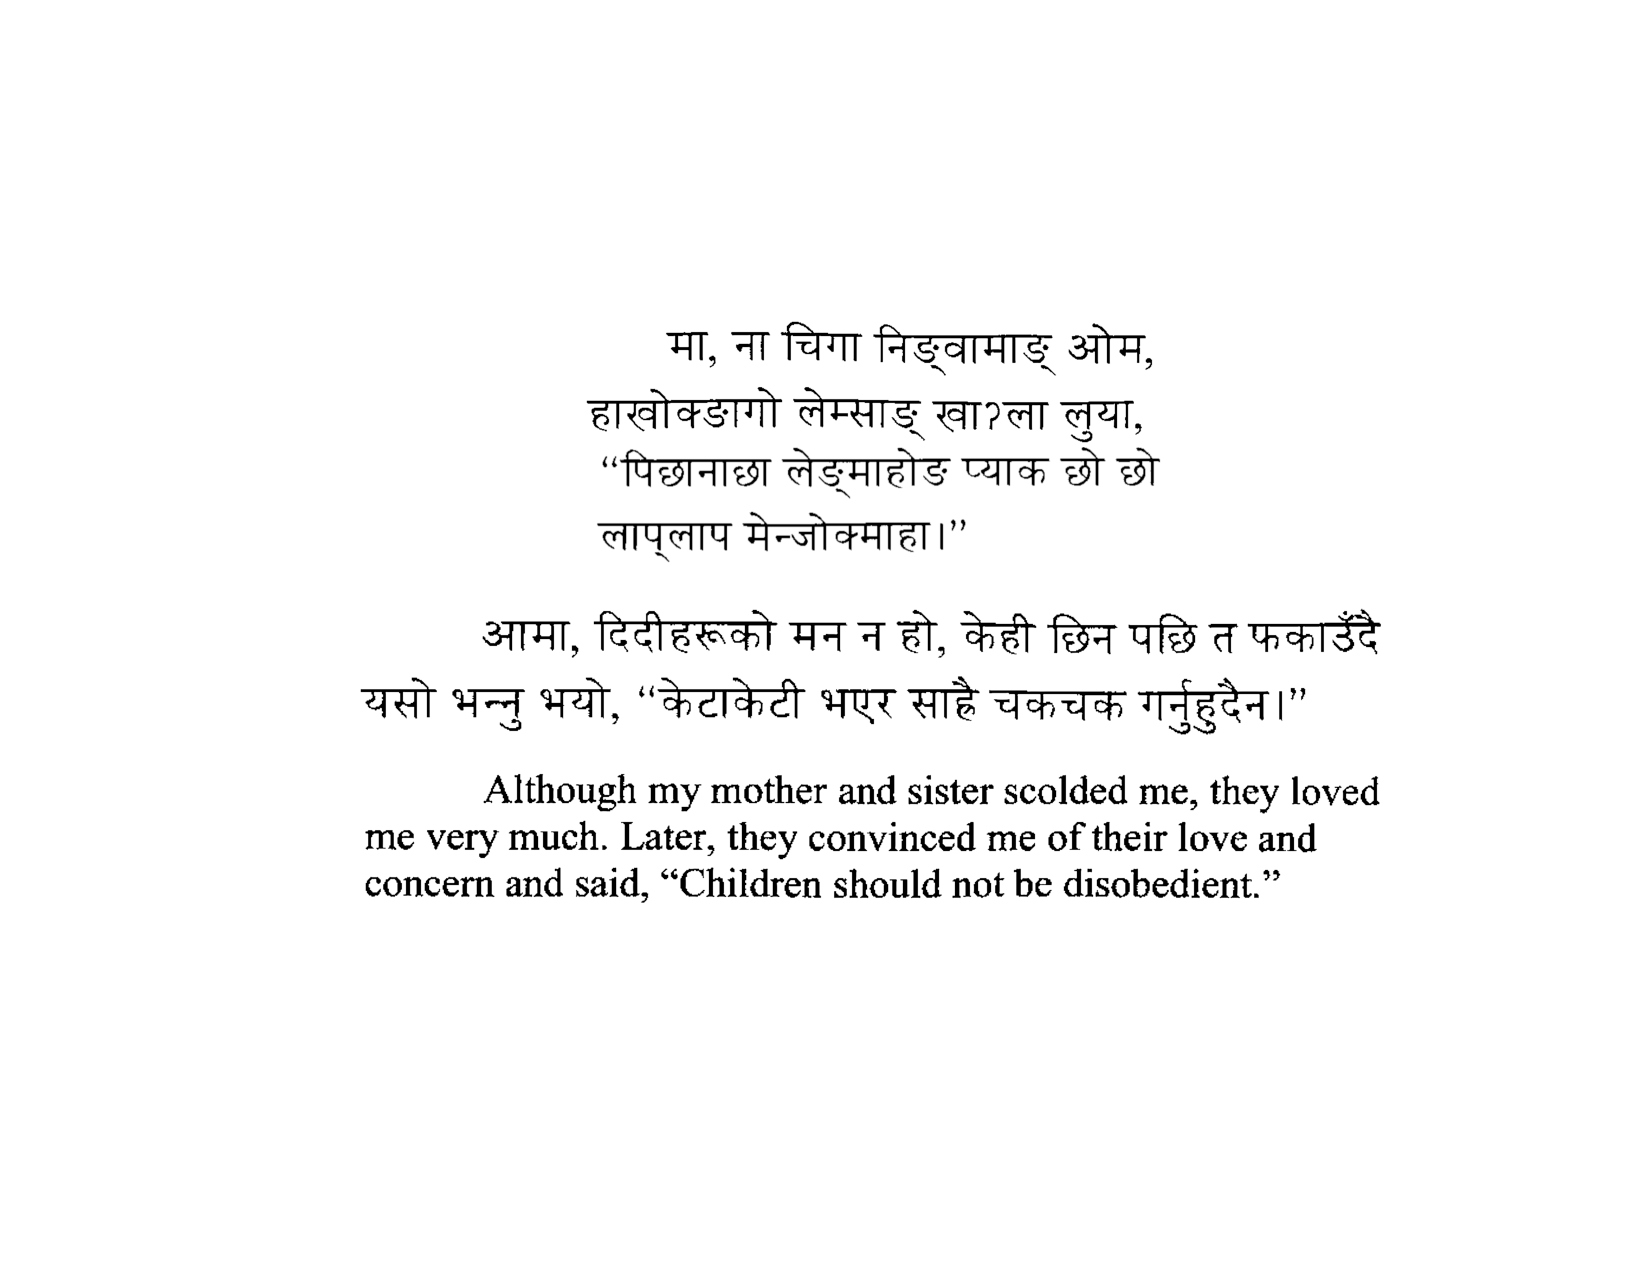
\includegraphics[width=0.9\columnwidth]{images/figure2c.pdf}}
      \vspace{0.6em}
    \end{subfigure}
    \footnotesize{(d) Handwritten Shangaji -- typed English glosses}
    \begin{tabular}{|@{\ \ }c@{\ \ }|}
    \hline
     \begin{subfigure}[t]{0.9\columnwidth}
      \centering
      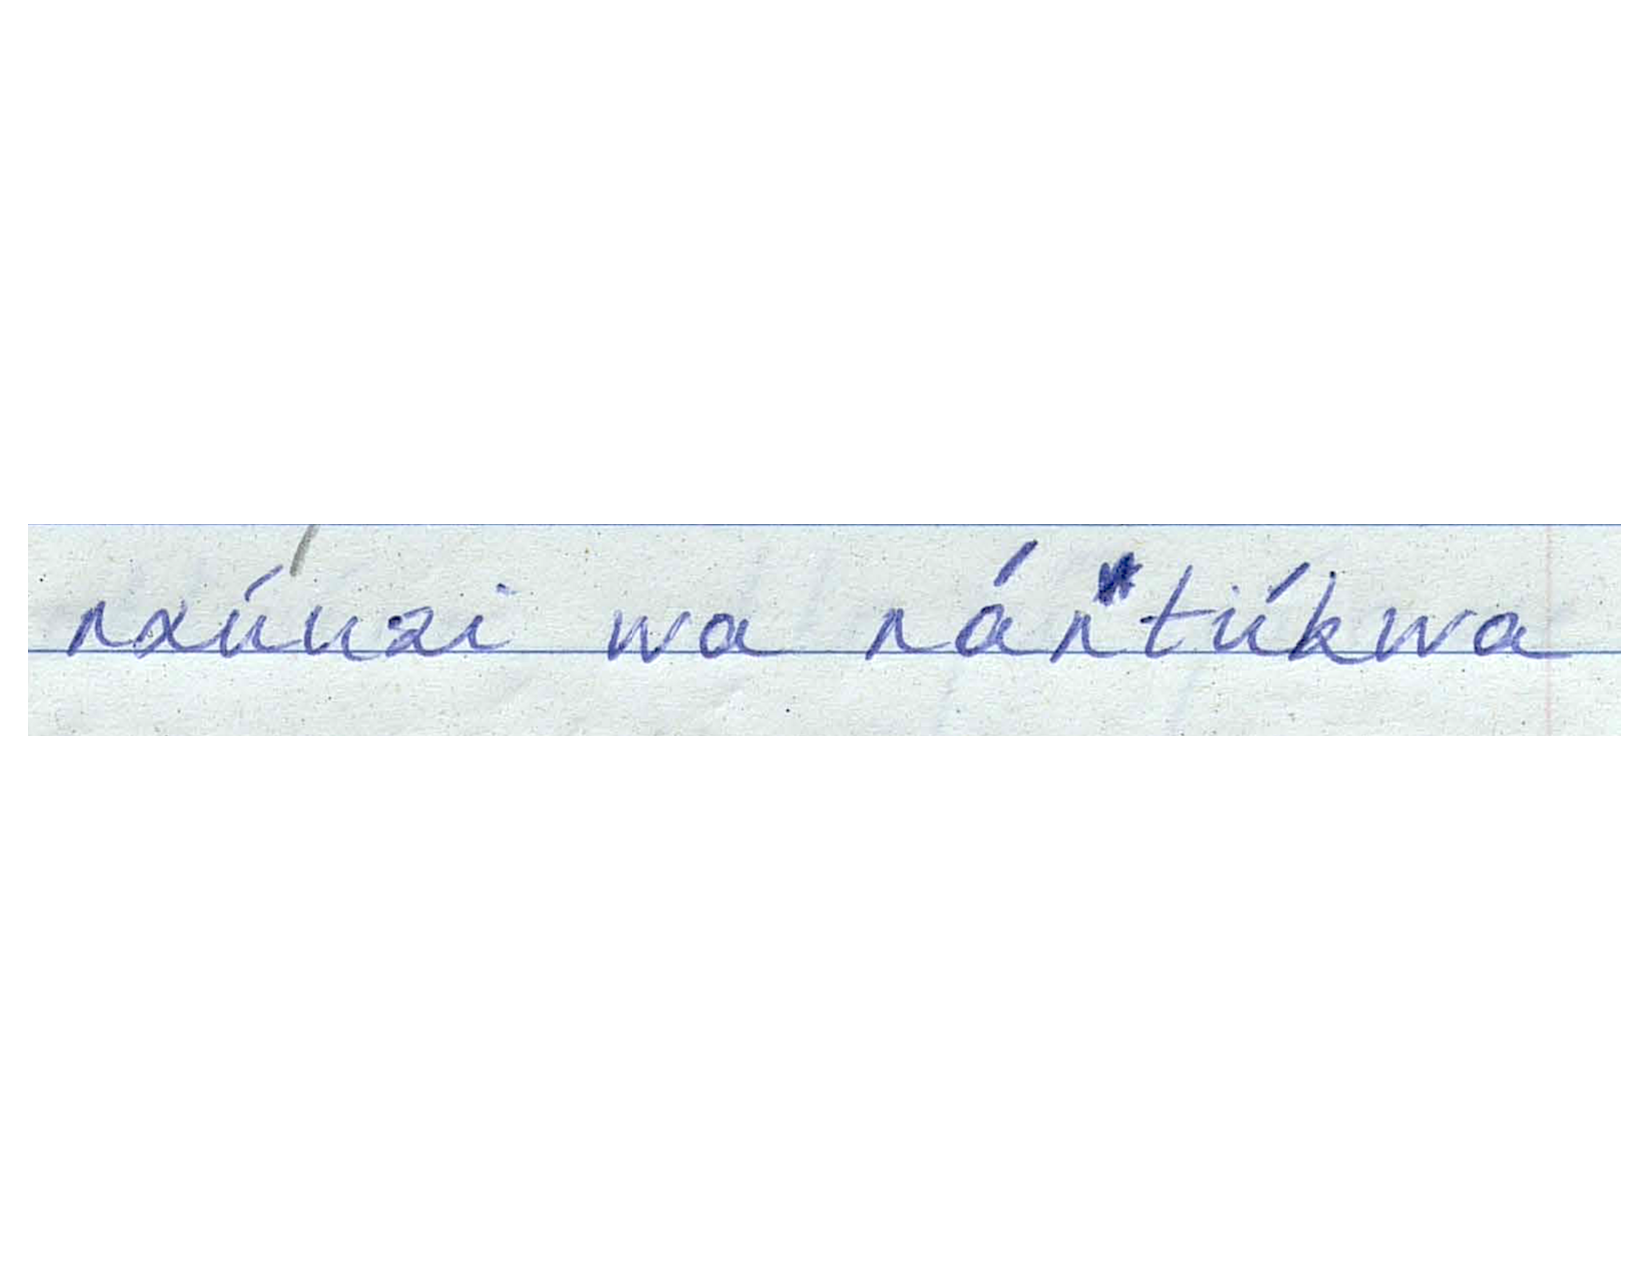
\includegraphics[width=0.9\columnwidth]{images/sha_img.pdf}
      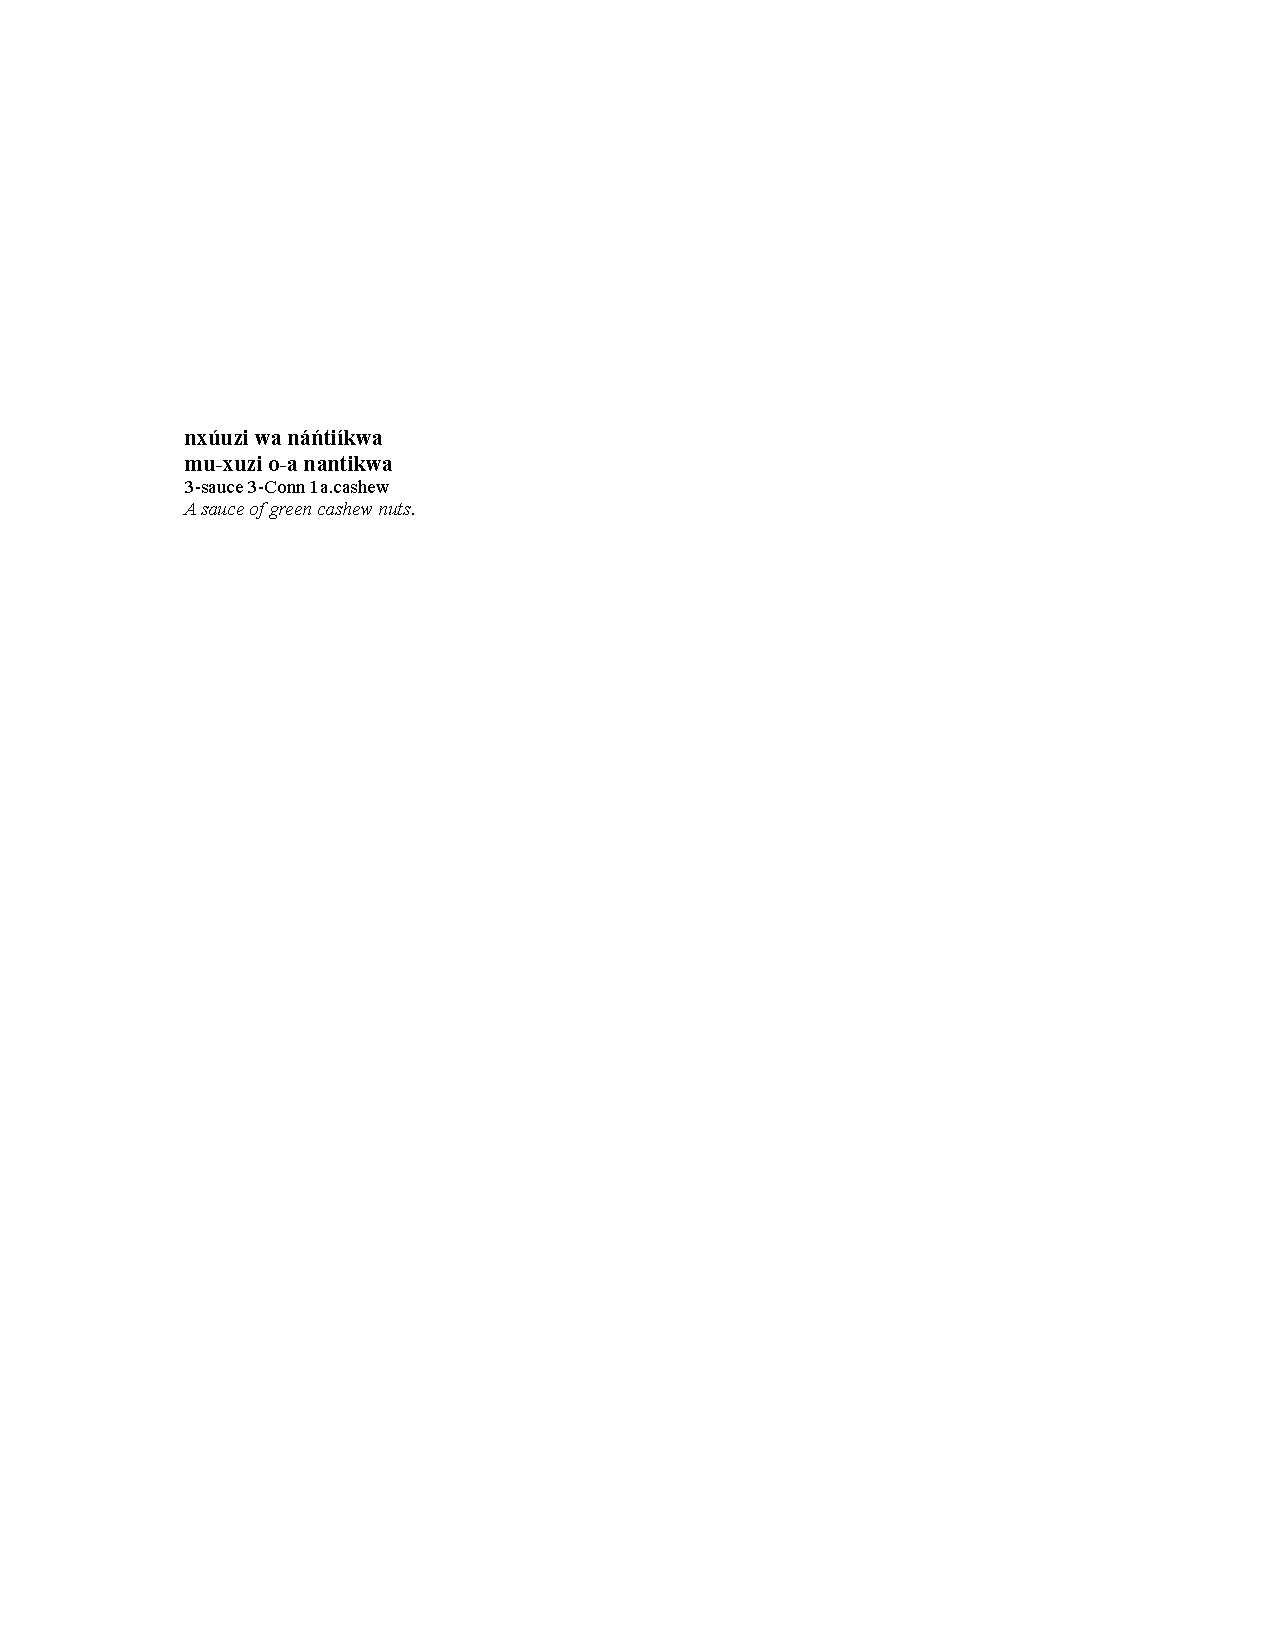
\includegraphics[width=0.5\columnwidth]{images/sha_text.pdf}
    \end{subfigure}\\
    \hline
    \end{tabular}
    \caption{Examples of scanned documents in endangered languages accompanied by translations from the same scanned book (a, b, c) or linguistic archive (d).}
    \label{fig:dataset_example}
    \vspace{-1.2em}
\end{figure}

Natural language processing (NLP) systems exist for a small fraction of the world's over 6,000 living languages, the primary reason being the lack of resources required to train and evaluate models. Technological advances are concentrated on languages that have readily available data, and most other languages are left behind~\cite{joshi2020state}. This is particularly notable in the case of endangered languages, i.e., languages that are in danger of becoming extinct due to dwindling numbers of native speakers and the younger generations shifting to using other languages. For most endangered languages, finding \emph{any} data at all is challenging.

In many cases, natural language text in these languages does exist. However, it is locked away in formats that are not machine-readable --- paper books, scanned images, and unstructured web pages. These include books from local publishing houses within the communities that speak endangered languages, such as educational or cultural materials. Additionally, linguists documenting these languages also create data such as word lists and interlinear glosses, often in the form of handwritten notes. Examples from such scanned documents are shown in~\autoref{fig:dataset_example}. Digitizing the textual data from these sources will not only enable NLP for endangered languages but also aid linguistic documentation, preservation, and accessibility efforts.

In this work, we create a benchmark dataset and propose a suite of methods to extract data from these resources, focusing on scanned images of paper books containing endangered language text. Typically, this sort of digitization requires an optical character recognition (OCR) system. However, the large amounts of textual data and transcribed images needed to train state-of-the-art OCR models from scratch are unavailable in the endangered language setting. Instead, we focus on \emph{post-correcting} the output of an off-the-shelf OCR tool that can handle a variety of scripts. We show that targeted methods for post-correction can significantly improve performance on endangered languages.

Although OCR post-correction is relatively well-studied, most existing methods rely on considerable resources in the target language, including a substantial amount of textual data to train a language model~\cite{schnober-etal-2016-still,dong-smith-2018-multi,8978127} or to create synthetic data~\cite{krishna-etal-2018-upcycle}. While readily available for high-resource languages, these resources are severely limited in endangered languages, preventing the direct application of existing post-correction methods in our setting. 

As an alternative, we present a method that compounds on previous models for OCR post-correction, making three improvements tailored to the data-scarce setting. First, we use a \textbf{multi-source model} to incorporate information from the high-resource translations that commonly appear in endangered language books. These translations are usually in the \textit{lingua franca} of the region (e.g., \autoref{fig:dataset_example} (a,b,c)) or the documentary linguist's primary language (e.g., \autoref{fig:dataset_example} (d) from \citet{shangaji-elar}). Next, we introduce \textbf{structural biases} to ease learning from small amounts of data. Finally, we add \textbf{pretraining methods} to utilize the little unannotated data that exists in endangered languages.

\medskip
\noindent
We summarize our main contributions as follows:
\begin{itemize}[leftmargin=*, itemsep=3pt]
    \item A benchmark dataset for OCR post-correction on three critically endangered languages: Ainu, Griko, and Yakkha.
    \item A systematic analysis of a general-purpose OCR system, demonstrating that it is not robust to the data-scarce setting of endangered languages.
    \item An OCR post-correction method that adapts the standard neural encoder-decoder framework to the highly under-resourced endangered language setting, reducing both the character error rate and the word error rate by 34\% over a state-of-the-art general-purpose OCR system.
\end{itemize}
